\PassOptionsToPackage{table}{xcolor}
\documentclass[9pt,xcolor=x11names,compress]{beamer}

%% General document %%%%%%%%%%%%%%%%%%%%%%%%%%%%%%%%%%
\usepackage{graphicx}
\usepackage{tikz}
\usetikzlibrary{decorations.fractals,lindenmayersystems}
\usepackage{wasysym}
%%%%%%%%%%%%%%%%%%%%%%%%%%%%%%%%%%%%%%%%%%%%%%%%%%%%%%


%% Beamer Layout %%%%%%%%%%%%%%%%%%%%%%%%%%%%%%%%%%
\useoutertheme[subsection=false,shadow]{miniframes}
\useinnertheme{default}
\usefonttheme{serif}
\usepackage{palatino}

\setbeamerfont{title like}{shape=\scshape}
\setbeamerfont{frametitle}{shape=\scshape}

\setbeamercolor*{lower separation line head}{bg=DeepSkyBlue4} 
\setbeamercolor*{normal text}{fg=black,bg=white} 
\setbeamercolor*{alerted text}{fg=DeepSkyBlue4} 
\setbeamercolor*{example text}{fg=black} 
\setbeamercolor*{structure}{fg=black} 
 
\setbeamercolor*{palette tertiary}{fg=black,bg=black!10} 
\setbeamercolor*{palette quaternary}{fg=black,bg=black!10} 

\setbeamertemplate{blocks}[rounded][shadow=true]
\setbeamercolor{block title}{bg=DeepSkyBlue4}
\setbeamercolor{block title example}{bg=DeepSkyBlue4}
\setbeamercolor{block body}{bg=black!15!white}
\setbeamercolor{block body example}{bg=black!15!white}

\setbeamertemplate{navigation symbols}{}
%%%%%%%%%%%%%%%%%%%%%%%%%%%%%%%%%%%%%%%%%%%%%%%%%%

\title{Lesson 6: Exponential Growth and Decay}
\author[Francisco Blanco-Silva]{Francisco Blanco-Silva}
\institute[USC]{University of South Carolina}
\date{
	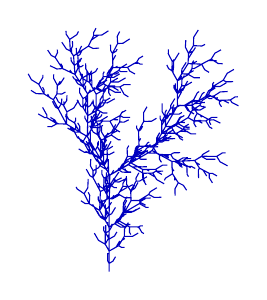
\begin{tikzpicture} 
    \draw [blue!75!black, rotate=90]
    [l-system={rule set={F -> FF-[-F+F]+[+F-F]}, axiom=F, order=4, step=2pt, 
        randomize step percent=25, angle=30, randomize angle percent=15}]
    lindenmayer system; 
	\end{tikzpicture}
}

\begin{document}

\frame{\titlepage}

\section{What do we know?}
\begin{frame}
\frametitle{What do we know?}
\begin{columns}[T]
\begin{column}{0.6\linewidth}
\begin{itemize}
\item Functions
\begin{itemize}
\item $x-$ and $y-$intercepts ($f(x)=0$, $f(0)$)
\item Change from $x=a$ to $x=b$ 
\begin{equation*}
	\Delta y = f(b)-f(a)
\end{equation*}
\item Average Rate of Change from $x=a$ to $x=b$
\begin{equation*}
ARC=\frac{\Delta y}{\Delta x}=\frac{f(b)-f(a)}{b-a} 
\end{equation*}
\item Relative Change from $x=a$ to $x=b$
\begin{equation*}
RC=\frac{\Delta y}{f(a)}=\frac{f(b)-f(a)}{f(a)}
\end{equation*}
\end{itemize}
\end{itemize}
\end{column}
\begin{column}{0.4\linewidth}
\begin{itemize}
	\item Linear Functions: $f(x)=b+mx$
	\item Exponential Functions $P_0 a^t = P_0 (1+r)^t = P_0 e^{kt}$
	\begin{align*}
	\uncover<2->{a&=1+r &r&=a-1 \\}
	\uncover<3->{k&=\ln a &a&=e^k \\}
	\uncover<4->{r&=	e^k-1 &k&=\ln(1+r)}
	\end{align*}
\end{itemize}
\end{column}
\end{columns}
\end{frame}

\section{Exponential Growth and Decay}

\begin{frame}[c]\frametitle{Exponential Growth and Decay}
    
\framesubtitle{How do we recognize it?}

\begin{itemize}[<+->]
  \item If the function is in the form $P = P_0 a^t$, $a>1$ gives exponential growth, and $a<1$ gives exponential decay.
  \item If the function is in the form $P = P_0 (1+r)^t$, $r>0$ gives exponential growth, and $r<0$ gives exponential decay.
  \item If the function is in the form $P = P_0 e^{kt}$, $k>0$ gives exponential growth, and $k<0$ gives exponential decay.
\end{itemize}
\end{frame}

\subsection{Examples}
\begin{frame}[t]\frametitle{Exponential Growth and Decay}
\framesubtitle{Examples}
\begin{example}
	The EPA investigated a spill of radioactive iodine.  The radiation level at site was 2.4 milirems/hour.  The level of radiation \alert{decays} at a \alert{continuous hourly rate} of $k=-0.04$.
	\begin{itemize}
		\item \alert<2>{What was the level of radiation 24 hours later?}
		\item \alert<3->{Find the number of hours until the level of radiation reached the maximum acceptable limit (0.6 milirems/hour).}
	\end{itemize}
\end{example}
	\only<2-4>{
   We need to find a function that models this situation.  The problem suggests that we need an exponential function, for which we know its continuous decay rate ($k=-0.04$) and its initial value ($P_0=2.4$)
	\begin{align*}
		\uncover<3->{P&=P_0 e^{kt}=2.4 e^{-0.04 t} (\text{in milirems/hour}) &t&=\text{ hours after}}
	\end{align*}
  \uncover<4->{
	The first question is asking for the radiation level after 24 hours:
	\begin{equation*}
	P(24)=2.4 e^{-0.04 \times 24}=0.9189429264 \text{ milirems/hour}
	\end{equation*}}}
  \only<5->{
   We need to solve for $t$ in the equation $P(t)=0.6$
  \begin{align*}
    P(t) &= 0.6 \\
    \uncover<4->{2.4 e^{-0.04 t} &= 0.6 \\}
    \uncover<5->{e^{-0.04 t} &= \frac{0.6}{2.4} = 0.25} \uncover<8->{&\alert{t}&\alert{= \frac{-1.386294361}{-0.04} \approx 34.65735903 \text{ hours.}}}\\
    \uncover<6->{\ln e^{-0.04 t} &= \ln 0.25 \\}
    \uncover<7->{-0.04 t &= -1.386294361 }
  \end{align*}}
\end{frame}

\section{Doubling time, half-life}
\subsection{Definitions}
\begin{frame}\frametitle{Doubling-time, Half-life}
    
\begin{definition}
  The \alert{doubling-time} of an exponentially increasing quantity is the time required for the quantity to double.
  \begin{align*}
    \uncover<2->{P(t) &= 2P_0} \uncover<5->{&\ln e^{kt} &= \ln 2 \\}
    \uncover<3->{P_0 e^{kt} &= 2P_0} \uncover<6->{&kt &= \ln 2 \\}
    \uncover<4->{e^{kt} &= 2} \uncover<7->{& \alert{t} &\alert{= \frac{\ln 2}{k} }}
  \end{align*}
  \pause\pause\pause\pause\pause\pause\pause The \alert{half-life} of an exponentially decreasing quantity is the time required for the quantity to be reduced by a factor of one half.
  \begin{align*}
    \uncover<9->{P(t) &= \tfrac{1}{2} P_0} \uncover<12->{& \ln e^{kt} &= \ln \tfrac{1}{2} \\}
    \uncover<10->{P_0 e^{kt} &= \tfrac{1}{2} P_0} \uncover<13->{&kt &= -\ln 2\\}
    \uncover<11->{e^{kt} &= \tfrac{1}{2}} \uncover<14->{& \alert{t} &\alert{= \frac{-\ln 2}{k}}}
  \end{align*}
\end{definition}
\end{frame}

\subsection{Examples}
\begin{frame}\frametitle{Doubing-time, Half-life}
\framesubtitle{Examples}
\begin{example}
  The quantity of ozone, $Q$, is decaying exponentially at a continuous rate of 0.25\% per year.   What is the half-life of the ozone?
\end{example}
\pause We use the formula directly.  We only need to know the value of the continuous decay rate, $k$, which is given to us: $k=-0.0025$. \uncover<2->{It is then
\begin{equation*}
t = \frac{-\ln 2}{k}  \uncover<3->{= \frac{-\ln 2}{-0.0025} \approx 277.25887224 \text{ years.}}
\end{equation*}}
\end{frame}

\section{Compound Interest}
\subsection{Definitions}
\begin{frame}\frametitle{Compound Interest}
An amount of money, $P_0$, is deposited in an account paying interest at a rate of $r$ per year.  Let $P$ be the balance in the account after $t$ years.  
\begin{itemize}
  \item If the interest is \alert{compounded annually}, then $P=P_0(1+r)^t$.
  \item If the interest is \alert{compounded continuously}, then $P=P_0e^{rt}$.
\end{itemize}
\pause
\begin{example}
  A bank advertises an interest rate of 8\% per year.  If you deposit \$5,000, how much is in the account 3 years later if the interest is compounded\dots
  \begin{itemize}
    \item \alert<3>{Annually?}
    \item \alert<4>{Continuously?}
  \end{itemize}
\end{example}
\begin{itemize}
  \item<3-> We use the formula $P(t)=P_0(1+r)^t$ here, with $r=0.08$, and $P_0=5000$.  We need to compute $P(3)$
  \begin{equation*}
    P(3) = 5000(1+0.08)^3= \$ 6298.56
  \end{equation*}
  \item<4-> We use the formula $P(t)=P_0e^{rt}$ for the same values of $r$ and $P_0$
  \begin{equation*}
    P(3)=5000e^{0.08 \times 3} = \$ 6356.24575
  \end{equation*}
\end{itemize}
\end{frame}

\subsection{Examples}
\begin{frame}\frametitle{Compound Interest}
\framesubtitle{Examples}
\begin{block}{Future Value}
  If \$10,000 is deposited in an account paying interest at a rate of 5\% per year, compounded continuously, how long does it take for the balance in the account to reach \$15,000?
\end{block}
\pause We have to solve for $t$ in the equation $P(t)=15000$, where $P=P_0e^{rt}$.  They are giving us $P_0=10000$ and $r=0.05$:
\begin{align*}
  \uncover<3->{P(t) &= 15000} \uncover<7->{& 0.05 t &= 0.4054651081 \\}
  \uncover<4->{10000e^{0.05 t} &= 15000} \uncover<8->{& t &= \frac{0.4054651081}{0.05} \\}
  \uncover<5->{e^{0.05 t} &= \frac{15000}{10000}} \uncover<9->{& \alert{t} &\alert{\approx 8.109302162 \text{ years}} \\}
  \uncover<6->{\ln e^{0.05 t} &= \ln 1.5 \\}
\end{align*}

\uncover<10->{That is a little bit more than eight years and one month (1.31163 months)}

\uncover<11->{Or better, eight years and almost six weeks (5.70311 weeks)}

\uncover<12->{Or even better, eight years almost 40 days (39.9218 days)}
\end{frame}

\begin{frame}\frametitle{Compound Interest}
\framesubtitle{Examples}
\begin{block}{Future Value}
 You win the lottery and are offered the choice between \$1 million  in four yearly installments of \$250,000 each, starting now, or a lump-sum payment of \$920,000 now. 

 Assuming a 6\% interest rate per year, compounded continuously, and ignoring taxes, which should you choose?
\end{block}
\pause  The following table summarizes the two situations:
\begin{center}
\begin{tabular}{|l|r|r|r|r|}
\hline
& 2015 & 2016 & 2017 & 2018 \\
\hline
First option & 250,000 &&&\\
&& +250,000 & +250,000 & +250,000 \\
&&&&\\
\hline
Second option & 920,000 & & & \\
\hline
\end{tabular}
\end{center}
\end{frame}

\begin{frame}\frametitle{Compound Interest}
\framesubtitle{Examples}
\begin{center}
\begin{tabular}{|l|r|r|r|r|}
\hline
& 2015 & 2016 & 2017 & 2018 \\
\hline
First option & 250,000 & \alert<1>{265459} & \only<2->{\alert<2>{547333}} & \only<3->{\alert{846637}}\\
&& +250,000 & +250,000 & +250,000 \\
&&=\alert<1>{515459}& \only<2->{= \alert<2>{797333}} & \only<3->{=\alert{1096637}} \\
\hline
Second option & 920,000 & & & \\
\hline
\end{tabular}
\end{center}
Let us examine the first option.  
\begin{itemize}
\item In one year, the initial amount of \$250,000 gives us $P(1)=250000e^{0.06 \times 1} = 265459.13675$ after compounding at 6\%. Then we add \$250,000 more, for a total of $265459.13675+250000=515459.13675$.

\item<2-> After another year, this amount increases to $P(1)=515459.13675e^{0.06}= 547333.34989$.  We add \$250,000 again, to obtain $547333.34989+250000=797333.34989$.

\item<3-> After another year, this amounts increases to $P(1)=797333.34989e^{0.06}=846637.69106$.  At that moment, we add the last \$250,000 to get the final amount of $846637.69106+250000=1096637.69106$
\end{itemize}
\end{frame}

\begin{frame}\frametitle{Compound Interest}
\framesubtitle{Examples}
\begin{center}
\begin{tabular}{|l|r|r|r|r|}
\hline
& 2015 & 2016 & 2017 & 2018 \\
\hline
First option & 250,000 & 265459 & 547333 & 846637\\
&& +250,000 & +250,000 & +250,000 \\
&&&& =\alert{1096637} \\
\hline
Second option & 920,000 & & & \alert{1101439}\\
\hline
\end{tabular}
\end{center}
Let us examine the second option.  We only need to worry about how much we have after 3 years:
\begin{equation*}
  P(3)=920000e^{0.06 \times 3} = 1101439.974
\end{equation*}
Which option do you prefer?
\end{frame}
\end{document}